\documentclass[a4paper]{article}
\usepackage{graphicx}
\usepackage{amsmath}
\usepackage{subcaption}
\usepackage{geometry}
\usepackage{adjustbox}
\usepackage[table]{xcolor}
\usepackage{array}
\usepackage[pages=all, color=black, position={current page.south}, placement=bottom, scale=1, opacity=1, vshift=5mm]{background}
\usepackage[margin=1in]{geometry} % full-width

% AMS Packages
\usepackage{amsmath}
\usepackage{amsthm}
\usepackage{amssymb}

% Unicode
\usepackage[utf8]{inputenc}
\usepackage{hyperref}
\hypersetup{
	unicode,
%	colorlinks,
%	breaklinks,
%	urlcolor=cyan, 
%	linkcolor=blue, 
	pdfauthor={Author One, Author Two, Author Three},
	pdftitle={A simple article template},
	pdfsubject={A simple article template},
	pdfkeywords={article, template, simple},
	pdfproducer={LaTeX},
	pdfcreator={pdflatex}
}

% Vietnamese
%\usepackage{vntex}

% Natbib
\usepackage[sort&compress,numbers,square]{natbib}
\bibliographystyle{mplainnat}

% Theorem, Lemma, etc
\theoremstyle{plain}
\newtheorem{theorem}{Theorem}
\newtheorem{corollary}[theorem]{Corollary}
\newtheorem{lemma}[theorem]{Lemma}
\newtheorem{claim}{Claim}[theorem]
\newtheorem{axiom}[theorem]{Axiom}
\newtheorem{conjecture}[theorem]{Conjecture}
\newtheorem{fact}[theorem]{Fact}
\newtheorem{hypothesis}[theorem]{Hypothesis}
\newtheorem{assumption}[theorem]{Assumption}
\newtheorem{proposition}[theorem]{Proposition}
\newtheorem{criterion}[theorem]{Criterion}
\theoremstyle{definition}
\newtheorem{definition}[theorem]{Definition}
\newtheorem{example}[theorem]{Example}
\newtheorem{remark}[theorem]{Remark}
\newtheorem{problem}[theorem]{Problem}
\newtheorem{principle}[theorem]{Principle}

\usepackage{graphicx, color}
\graphicspath{{fig/}}

%\usepackage[linesnumbered,ruled,vlined,commentsnumbered]{algorithm2e} % use algorithm2e for typesetting algorithms
\usepackage{algorithm, algpseudocode} % use algorithm and algorithmicx for typesetting algorithms
\usepackage{mathrsfs} % for \mathscr command

\usepackage{lipsum}

% Author info
\title{ \textbf{Machine Learning Approaches for Effective Movie Recommendations: A Comprehensive Study} }
\author{Aditya Sahani$^1$ \and  Arjun Bhattad$^2$ \and Raunak Singh$^3$  \and  Krishna Chaudhary$^4$}

\date{
	Indian Institute of Technology, Jodhpur \\ \texttt{\{b22cs003, b22ai051, b22cs085, b22ee090\}@iitj.ac.in}\\%
	[2ex]%
%	\today
}

% Redefining the abstract environment to make the heading bigger
\renewenvironment{abstract}
 {\Large\textbf{Abstract}\vspace{0.5em}\par\noindent\ignorespaces}
 {\par\vspace{0.5em}}

\begin{document}
	\maketitle
	
	\begin{abstract}
{\fontsize{11}{15}\selectfont
In this project, we have developed a comprehensive movie recommendation system integrating various techniques including content-based, collaborative filtering, and hybrid models. Leveraging state-of-the-art machine learning and natural language processing algorithms, our system provides personalized movie recommendations tailored to individual user preferences.

The content-based approach analyzes movie features such as genre, director, and synopsis to recommend similar movies based on their content characteristics. Collaborative filtering techniques utilize user-item interactions and similarities among users or items to make recommendations. Additionally, hybrid models combine the strengths of both content-based and collaborative filtering methods to enhance recommendation accuracy and coverage.

Our project encompasses data preprocessing, feature engineering, model training, and deployment phases. We have employed popular libraries such as Pandas, NumPy, Scikit-learn, and TensorFlow to build and evaluate the recommendation models. Through extensive experimentation and evaluation, we have optimized the system's performance, considering metrics such as accuracy, diversity, and scalability.

The deployed recommendation system offers a user-friendly interface where users can discover relevant movies based on their preferences and browsing history. Furthermore, continuous monitoring and updates ensure the system remains adaptive to evolving user tastes and preferences.

Overall, our project contributes to the advancement of recommendation systems by demonstrating the effectiveness of integrating multiple techniques to deliver personalized and engaging movie recommendations in real-world applications.}

		\vspace{2cm}	
		\noindent\textbf{Keywords:} content-based, collaborative, hybrid filtering
	\end{abstract}

	\tableofcontents
	\newpage
	\section{\LARGE Introduction}
	% \label{sec:intro}
	{ \fontsize{12}{15}\selectfont In today's digital age, the vast array of available content can be overwhelming for individuals seeking entertainment options. From movies and TV shows to books and music, the abundance of choices often leads to decision fatigue and frustration. In response to this challenge, recommendation systems have emerged as invaluable tools, designed to alleviate the burden of choice by offering personalized suggestions tailored to individual preferences and interests.

 In the realm of movies, recommendation systems play a pivotal role in helping users discover new films that align with their tastes and preferences. By harnessing the collective wisdom of user data and sophisticated machine learning techniques, these systems offer a curated selection of movies that are not only interesting but also likely to resonate with the individual user. Whether it's uncovering hidden gems, exploring niche genres, or staying up-to-date with the latest releases, recommendation systems empower users to navigate the vast cinematic landscape with ease and confidence.

 Through this project, different machine learning approaches are harnessed to develop content-based, collaborative-based and hybrid-based recommender systems. Implementation of different models like
 \textbf{cosine similarity, matrix factorization} were done on MovieLens dataset to demonstrate the recommender systems. Evaluation of differnt models were done through \textbf{RMSE, MAE} and various plots.
 }
	
	\subsection{\Large Citing paper}
 
	\bibliography{ref}
    \cite{serrano_academy_2018}
    \cite{albakri2019collaborative}
    \cite{jacksonwu2019improving}
    \cite{ramyavidiyala2020how}
    \cite{sciforce2021deep}
    \cite{zhang2018deep}

 
\newpage
 \subsection{\Large Figures}
 
 \begin{figure}[h]
    \centering
    \begin{subfigure}{0.5\textwidth}
        \centering
        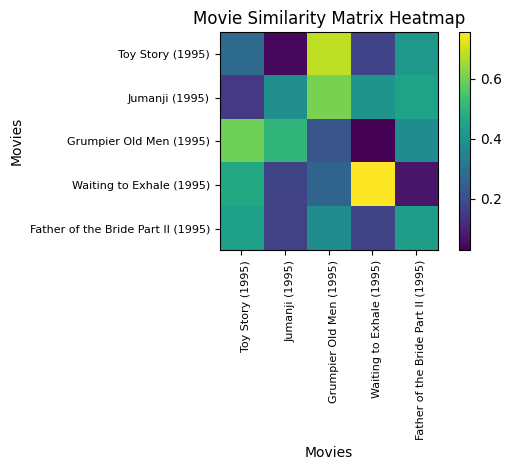
\includegraphics[width=0.5\textwidth]{./Figs/cosine_heatmap.png}
        \caption{HeatMap to show similarity between different movies.}
    \end{subfigure}%
    \begin{subfigure}{0.5\textwidth}
        \centering
        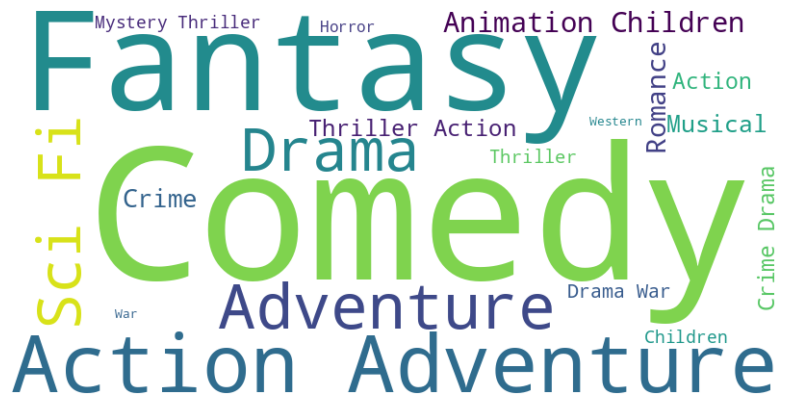
\includegraphics[width=0.9\textwidth, frame]{Figs/genres.png}
        \caption{WordCloud showing different genres in dataset.}
    \end{subfigure}

    \begin{subfigure}{\textwidth} % Modified width for the last image
        \centering
        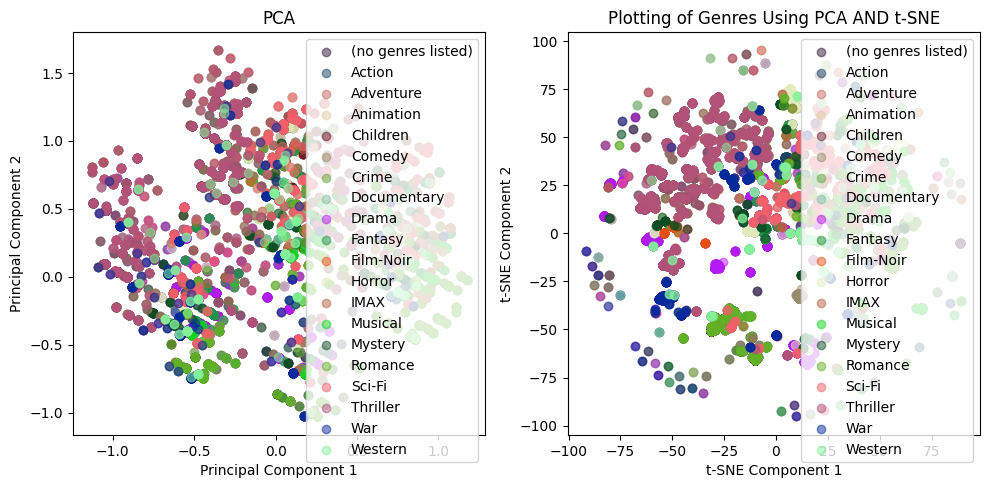
\includegraphics[width=0.5\textwidth, frame]{Figs/genres_pca.png} % Adjusted width to occupy whole width of the page
        \caption{Plotting genres using PCA and t-SNE.}
    \end{subfigure}

     \begin{subfigure}{\textwidth} % New subfigure for the additional image
        \centering
        \includegraphics[width=0.5\textwidth]{Figs/ratings_distribution.png}
        \caption{Ratings distribution Plot}
    \end{subfigure}
    
    \caption{Overall Analysis of Dataset}
\end{figure}
%  \begin{figure}[h]	
%     \begin{subfigure}{0.5\textwidth}
%         \centering
%         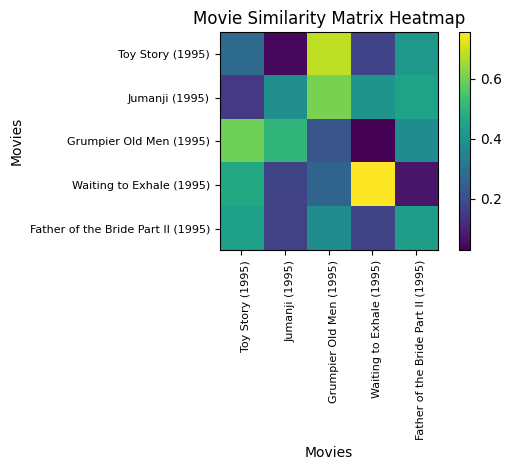
\includegraphics[width=8cm, height=8cm\textwidth]{./Figs/cosine_heatmap.png}
%         \caption{HeatMap to show similarity b/w different movies.}
%     \end{subfigure}%
%     \begin{subfigure}{0.5\textwidth}
%         \centering
%         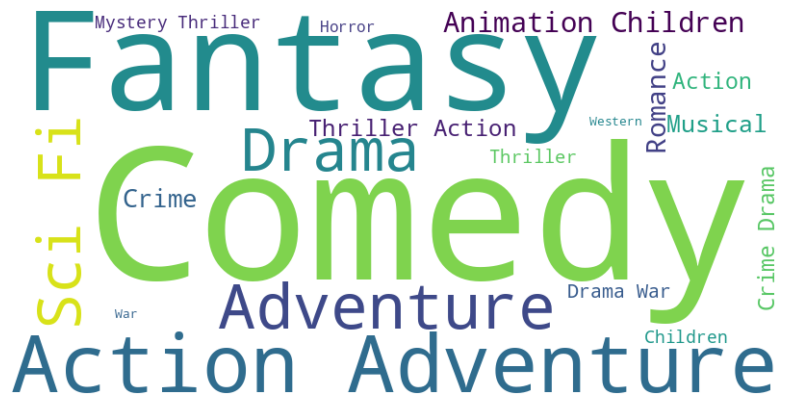
\includegraphics[width=8cm, height=8cm,frame\textwidth]{./Figs/genres.png}
%         \caption{WordCloud showing differnt genres in dataset.}
%     \end{subfigure}%


%     \begin{subfigure}{0.5\textwidth}
%         \centering
%         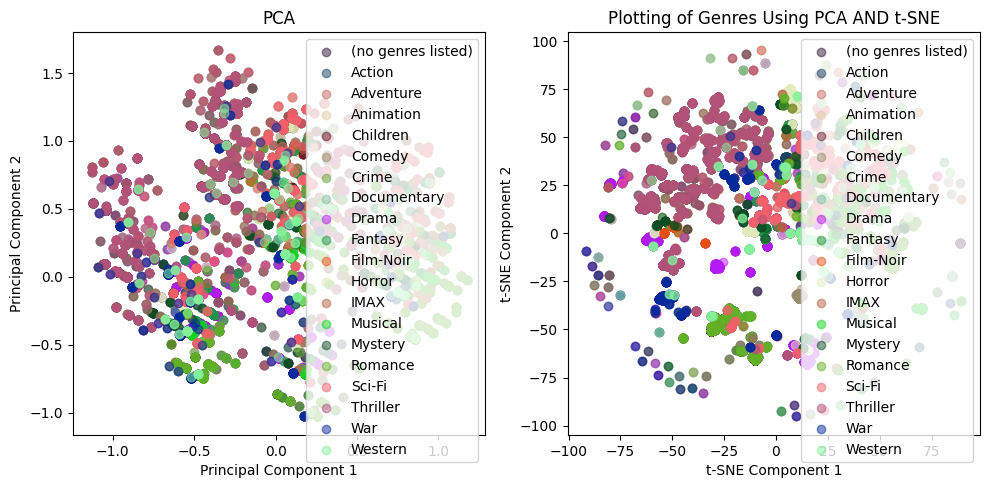
\includegraphics[width=0.9,frame\textwidth]{./Figs/genres_pca.png}
%         \caption{Plotting genres using PCA and t-SNE.}
%     \end{subfigure}%
    
%     \caption{Overall Analysis of Problem}
% \end{figure}

% \begin{figure}[h]
%     \begin{subfigure}{0.5\textwidth}
%         \centering
%         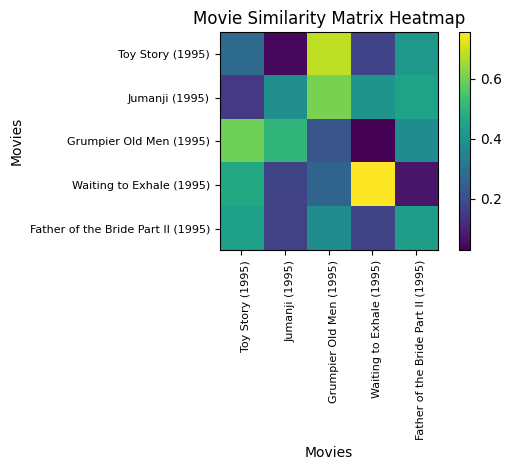
\includegraphics[width=8cm, height=8cm]{./Figs/cosine_heatmap.png}
%         \caption{HeatMap to show similarity between different movies.}
%     \end{subfigure}%
%     \begin{subfigure}{0.5\textwidth}
%         \centering
%         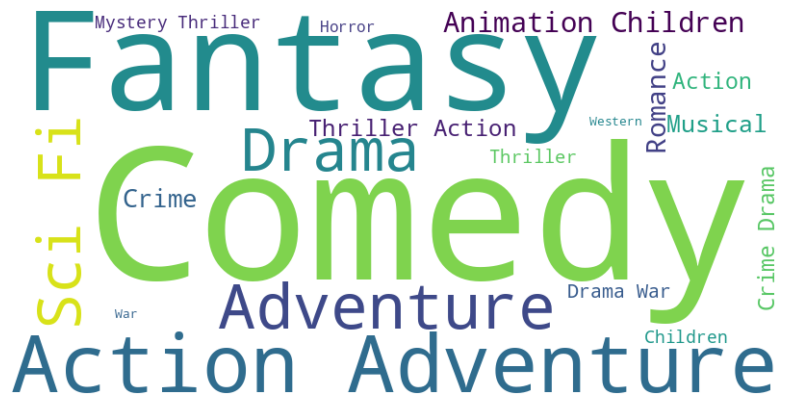
\includegraphics[width=8cm, height=8cm, frame]{./Figs/genres.png}
%         \caption{WordCloud showing different genres in dataset.}
%     \end{subfigure}

%     \begin{subfigure}{0.5\textwidth}
%         \centering
%         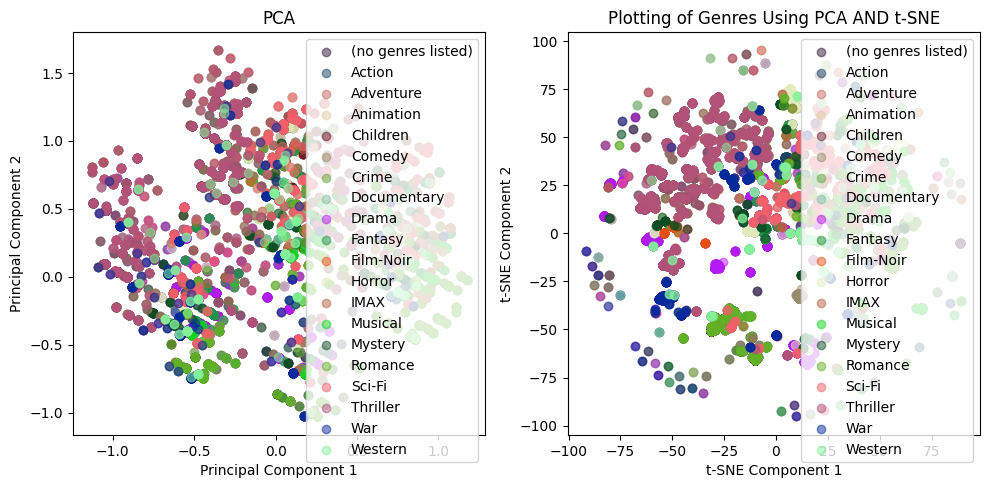
\includegraphics[width=2.0\textwidth, frame]{./Figs/genres_pca.png}
%         \caption{Plotting genres using PCA and t-SNE.}
%     \end{subfigure}
%     \caption{Overall caption for the figure}
% \end{figure}






% Approaches tried
	\newpage
	
\section{\LARGE Approaches Tried}
\label{sec:app}

\textbf{\Large Content-Based Filtering:}
\bigskip


Content-based filtering recommends items based on the attributes or features of the items themselves. It analyzes the properties or characteristics of items that users have interacted with in the past to recommend similar items. In the context of movie recommendation systems, content-based filtering compares the attributes of movies, such as genre, cast, director, and plot summary, to identify movies that are similar to those that a user has liked previously. This approach focuses on item characteristics rather than user interactions or preferences.

\bigskip

\textbf{\large \color[RGB]{50,50,50} Cosine Similarity:}



Cosine similarity is a metric used to measure the similarity between two vectors by calculating the cosine of the angle between them. In the context of movie recommendation systems, cosine similarity compares the feature vectors representing movies based on attributes such as genre, cast, director, etc. It quantifies how similar two movies are in terms of their attributes, allowing the system to recommend movies that are most similar to those that a user has liked in the past.


The cosine similarity between two vectors $A$ and $B$ is calculated as follows:
\[
\text{cosine\_similarity}(A, B) = \frac{{A \cdot B}}{{\|A\| \cdot \|B\|}}
\]
Where:
\begin{itemize}
    \item $A$ and $B$ are the feature vectors of two items (movies).
    \item $A \cdot B$ denotes the dot product of $A$ and $B$.
    \item $\|A\|$ and $\|B\|$ represent the Euclidean norms of $A$ and $B$, respectively.
\end{itemize}
\includegraphics[width=0.5\textwidth]{Figs/cosine_similarity.png}


\bigskip

\textbf{\large \color[RGB]{50,50,50} Jaccard Similarity:}


Jaccard similarity is a metric used to measure the similarity between two sets by comparing their intersection to their union. In movie recommendation systems, Jaccard similarity can be applied to compare sets of attributes associated with movies, such as genres, tags, or keywords. It quantifies how similar two movies are based on their common attributes, enabling the system to recommend movies that share common characteristics with those that a user has liked in the past.


The Jaccard similarity between two sets $A$ and $B$ is calculated as follows:
\[
\text{jaccard\_similarity}(A, B) = \frac{{|A \cap B|}}{{|A \cup B|}}
\]
Where:
\begin{itemize}
    \item $|A \cap B|$ denotes the size of the intersection of sets $A$ and $B$.
    \item $|A \cup B|$ represents the size of the union of sets $A$ and $B$.
\end{itemize}
\includegraphics[width=0.5\textwidth]{Figs/jaccard_similarity.jpg}

\bigskip


\textbf{\large \color[RGB]{50,50,50} K-Nearest Neighbors (KNN):}


K-Nearest Neighbors (KNN) is an algorithm used for recommendation by finding the $k$ nearest neighbors of a given item based on a similarity metric. In movie recommendation systems, KNN identifies the $k$ movies most similar to those that a user has liked in the past. This is achieved by calculating the similarity between movies using metrics such as cosine similarity or Euclidean distance, and then recommending movies that are closest to the user's liked items.


\bigskip

\textbf{\Large Collaborative Filtering:}
\bigskip


Collaborative filtering recommends items based on the preferences of other users. It analyzes user-item interactions and identifies users with similar preferences to recommend items that they have liked. In movie recommendation systems, collaborative filtering assumes that if a user has similar preferences to another user on certain items, they are likely to have similar preferences on other items as well. This approach focuses on leveraging the collective wisdom of users to make personalized recommendations.

\bigskip

\textbf{\large \color[RGB]{50,50,50} Deep Learning:}

Deep learning models, such as neural networks along with embeddings, can be used for collaborative filtering by learning complex patterns in user-item interactions from the data. They can capture nonlinear relationships between users and items, and predict the ratings which can be used to determine the next movie that user may watch.

\includegraphics[width=0.7\textwidth]{Figs/deep_lr.png}

\bigskip
\textbf{\large \color[RGB]{50,50,50} K-Means Clustering:}

K-Means clustering groups users or items into clusters based on their similarity. It can be used to segment users or items into groups with similar preferences, which can then be used for recommendation.

\includegraphics[width=0.6\textwidth]{Figs/k means clustering.png}

\bigskip
\textbf{\large \color[RGB]{50,50,50} Matrix Factorization:}


Matrix factorization decomposes the user-item interaction matrix into two lower-dimensional matrices representing latent factors for users and items. It captures underlying patterns in the data and can make recommendations based on these latent factors.

\includegraphics[width=0.7\textwidth]{Figs/matrix_factorization.png}

\bigskip
\textbf{\large \color[RGB]{50,50,50} Nearest Neighbors:}

Nearest neighbors-based collaborative filtering recommends items to a user based on the preferences of similar users or items. It finds users or items similar to the target user and recommends items liked by those similar users.


\bigskip
\textbf{\large \color[RGB]{50,50,50} Pearson Similarity:}

Pearson correlation measures the linear correlation between two variables, such as the ratings given by users to different items. In movie recommendation systems, Pearson similarity is used to find users with similar rating patterns and make recommendations based on their preferences. It quantifies how closely the ratings of two users align, enabling the system to identify users with similar tastes and recommend items liked by those users.


The Pearson correlation between two vectors $X$ and $Y$ is calculated as follows:
\[
\text{pearson\_correlation}(X, Y) = \frac{{\sum_{i=1}^{n}(X_i - \bar{X})(Y_i - \bar{Y})}}{{\sqrt{\sum_{i=1}^{n}(X_i - \bar{X})^2} \cdot \sqrt{\sum_{i=1}^{n}(Y_i - \bar{Y})^2}}}
\]
Where:
\begin{itemize}
    \item $X$ and $Y$ are vectors representing the ratings of two users on items.
    \item $X_i$ and $Y_i$ are the ratings of user $X$ and user $Y$ on item $i$, respectively.
    \item $\bar{X}$ and $\bar{Y}$ are the mean ratings of users $X$ and $Y$, respectively.
    \item $n$ is the number of items rated by both users.
\end{itemize}

\includegraphics[width=0.6\textwidth]{Figs/pearson_similarity.PNG}

\bigskip

\textbf{\Large Hybrid Filtering:}
\bigskip

Hybrid recommendation systems combine multiple recommendation techniques to improve recommendation accuracy and coverage. Here's the model you've implemented:

\bigskip
\textbf{\large \color[RGB]{50,50,50} Cosine Similarity and Matrix Factorization:}

This hybrid model combines content-based filtering (cosine similarity) and collaborative filtering (matrix factorization). It leverages both user-item interactions and item features to make recommendations, providing a more comprehensive approach to recommendation.



	
	\section{\LARGE Experiments and Results}
	\label{sec:app}
	Write about dataset, experimental setting, compare results

 \subsection{\Large \color[RGB]{50,50,50}  Dataset:}

 The MovieLens dataset is a widely used dataset in the field of recommender systems and movie recommendation research. It contains several CSV files:

\begin{itemize}
    \item \textbf{\Large movies.csv:} This file typically contains information about movies, such as movie IDs, titles, and genres. Each row represents a movie, and the columns might include movie ID, title, and genre information.

\begin{table}[htbp]
\centering
\caption{movies.csv}
\begin{tabular}{|c|c|c|c|}
\hline
index & movieId & title & genres \\
\hline
0 & 1 & Toy Story (1995) & Adventure| Animation|Children|Comedy|Fantasy \\
1 & 2 & Jumanji (1995) 	 & Adventure|Children|Fantasy \\
2 & 3 & Grumpier Old Men (1995) 	 & Comedy|Romance \\
\hline
\end{tabular}
\label{tab:my_table}
\end{table}
    
    \item \textbf{\Large ratings.csv:} This file contains user ratings for different movies. Each row typically represents a rating given by a user to a movie. Columns 
    may include user ID, movie ID, rating, and timestamp.
    
\begin{table}[htbp]
\centering
\caption{ratings.csv}
\begin{tabular}{|c|c|c|c|c|}
\hline
index & userId & movieId & rating & timestamp \\
\hline
0 & 1 & 1 & 4.0 & 964982703 \\
1 & 1 & 3 & 4.0 & 964981247 \\
2 & 1 & 6 & 4.0 & 964982224 \\
\hline
\end{tabular}
\label{tab:ratings.csv}
\end{table}
    
    \item \textbf{\Large links.csv:} This file contains additional metadata about movies, often including information to link the MovieLens dataset to other databases like IMDb. Columns may include movie ID, IMDb ID, and TMDB ID.

\begin{table}[htbp]
\centering
\caption{links.csv}
\begin{tabular}{|c|c|c|c|}
\hline
index & movieId & imdbId & tmdbId \\
\hline
0 & 1 & 114709 & 862.0 \\
1 & 2 & 113497 & 8844.0 \\
2 & 3 & 113228 & 15602.0 \\
\hline
\end{tabular}
\label{tab:links.csv}
\end{table}


    \item \textbf{\Large tags.csv:} This file contains user-generated tags for movies. Users can tag movies with different keywords or labels. Columns may include user ID, movie ID, tag, and timestamp.

\begin{table}[htbp]
\centering
\caption{tags.csv}
\begin{tabular}{|c|c|c|c|c|}
\hline
index & userId & movieId & tag & timestamp \\
\hline
0 & 2 & 60756 & funny & 1445714994 \\
1 & 2 & 60756 & Highly quotable & 1445714996 \\
2 & 2 & 60756 & will ferrell & 1445714992 \\
\hline
\end{tabular}
\label{tab:tags.csv}
\end{table}
\end{itemize}


% items ends
Combining information from these files, we build a recommendation system that utilizes various techniques such as content-based filtering (using movie attributes like genre or tags), collaborative filtering (based on user ratings), or hybrid approaches that combine both.

Important features from different dataset files are combined 
to form a new dataset which has the important columns, where we apply different models for recommender system.
% About dataset ends

% Preprocessing Techniques

\subsection{\Large \color[RGB]{50,50,50} Preprocessing:}
\begin{itemize}
    \item \textbf{Combining Important Features:} Merging relevant features from different datasets or files ensures that all necessary information is consolidated into a single dataset for analysis.
    \item \textbf{Combining Movie Title and Genres:} Combining movie titles and genres can provide a more comprehensive representation of movies, which is essential for content-based recommendation systems.
    \item \textbf{Word Tokenization:} Tokenizing the combined text splits it into individual words or tokens, making it easier to process and analyze.
    \item \textbf{Removing Punctuation:} Removing punctuation helps clean the text data and ensures consistency in the tokens.
    \item \textbf{Removing Stopwords:} Stopwords are common words like "the," "is," "and," etc., which do not contribute much to the mean
    \item \textbf{Removing Stem Words using Stemming:} Stemming reduces words to their root forms, which can help in consolidating similar words and reducing the vocabulary size.
    \item \textbf{Converting Text to Vectors:} Converting text data into numerical vectors is essential for machine learning algorithms to process the data. Techniques like \textbf{CountVectorizer and TF-IDF Vectorizer} convert text into numerical representations, where each word becomes a feature with a numerical value.
    \subsubsection{CountVectorizer : }
    CountVectorizer converts text into a numerical matrix, representing document-term frequency. For \( m \) documents and \( n \) unique words, it creates a \( m \times n \) matrix \( X \). Each cell \( X_{ij} \) holds the count \( n_{ij} \) of word \( j \) in document \( i \). This enables text data to be processed mathematically for machine learning tasks.
    
    \includegraphics[width=0.7\textwidth]{Figs/cv.png}

    \subsubsection{TF-IDF Vectorizer : }

    TF-IDF (Term Frequency-Inverse Document Frequency) is a technique used to quantify the importance of a word in a document relative to a collection of documents. For a word in a document:

\textbf{TF (Term Frequency)} measures how frequently a word appears in a document:
\[
TF_{ij} = \frac{n_{ij}}{\sum_k n_{ik}}
\]

\textbf{IDF (Inverse Document Frequency)} measures how important a word is across all documents:
\[
IDF_{j} = \log\left(\frac{N}{n_j}\right)
\]

Where:
\begin{itemize}
    \item \( n_{ij} \) is the count of word \( j \) in document \( i \).
    \item \( \sum_k n_{ik} \) is the total count of all words in document \( i \).
    \item \( N \) is the total number of documents.
    \item \( n_j \) is the number of documents containing word \( j \).
\end{itemize}

\textbf{TF-IDF} combines these measures to calculate the importance of a word:
\[
TF-IDF_{ij} = TF_{ij} \times IDF_{j}
\]

The higher the TF-IDF score, the more important the word is to the document.

    \item \textbf{Vector Representation of Text:} At the end of these preprocessing steps, we obtain a vector representation of text data, where each movie is represented by a numerical vector capturing its textual features. This vector representation is suitable for feeding into machine learning models for tasks like recommendation.   

    
\end{itemize}

Once the preprocessing part is done, we feed our text vectors into the different models like cosine similarity, pearson similarity to develop different kind of recommendation techniques.



% Preprocessing ends

% experiment begin

\subsection{\Large \color[RGB]{50,50,50} Experimentation:}
 \subsubsection{Content-Based Filtering : }
 
\begin{table}[htbp]
\centering
\begin{adjustbox}{max width=\textwidth}
\begin{tabular}{|p{3cm}|p{4.5cm}|p{4.5cm}|p{4.5cm}|}
\hline
\rowcolor{gray!20}
\textbf{Aspect} & \textbf{Cosine Similarity} & \textbf{Jaccard Similarity} & \textbf{KNN (K-Nearest Neighbors)} \\
\hline
Experimentation & Implemented cosine similarity for movie vectors. & Utilized Jaccard similarity for word sets. & Implemented KNN algorithm for movie vectors. \\
\hline
Advantages & 1.Robust to document length & 1. Effective for categorical data & 1.Considers entire feature space \\
 & 2.Computationally efficient & 2.Simple measure of similarity & 2.Captures complex relationships between movies \\
 & 3.Intuitive similarity scores &  &  \\
\hline
Disadvantages & 1.Limited semantic understanding & 1.Limited semantic understanding & 1.Suffers from curse of dimensionality \\
 & 2.May struggle with new or less popular movies & 2.Less nuanced recommendations & 2.Requires more computational resources \\
 &  &  & 3.May require tuning of hyperparameters \\
\hline
\end{tabular}
\end{adjustbox}
\caption{Comparison of Content-Based Recommendation Approaches}
\label{tab:comparison}
\end{table}

\newpage
 \subsubsection{Collaborative Filtering : }
 
\begin{table}[htbp]
\centering
\begin{adjustbox}{max width=\textwidth}
\begin{tabular}{|p{3cm}|p{4.5cm}|p{4.5cm}|p{4.5cm}|}
\hline
\rowcolor{gray!20}
\textbf{Aspect} & \textbf{Matrix Factorization} & \textbf{Pearson Similarity} & \textbf{K-Means} \\
\hline
Experimentation & Implemented matrix factorization to factorize user-item matrix. & Calculated Pearson correlation coefficient between users. & Utilized k-means clustering to group users or items. \\
\hline
Advantages & 1.Effective for handling sparse matrices & 1.Captures linear relationships between users & 1.Identifies user or item clusters \\
 & 2.Able to handle implicit feedback & 2.Robust to varying rating scales & 2.Scalable to large datasets \\
 & 3.Able to handle new users/items without retraining & 3.Provides personalized recommendations & 3.Can reveal latent user/item features \\
\hline
Disadvantages & 1.May suffer from overfitting & 1.Limited to linear relationships & 1.Requires specifying the number of clusters \\
 & 2.May require tuning hyperparameters & 2.Sensitive to outliers & 2.May produce inconsistent clusters \\
 & 3.Computationally intensive for large datasets & 3.Cold start problem for new users/items & 3.Interpretability may be challenging \\
\hline
\end{tabular}
\end{adjustbox}
\caption{Comparison of Collaborative Filtering Approaches}
\label{tab:collab_comparison}
\end{table}

\includegraphics[width=1\textwidth]{Figs/wcss.png}
Hence, from the graph we can see that optimum number of neighbours = \textbf{15 - 20}. Results are mentioned in section 3.4.

 \subsubsection{Hybrid Filtering : }
 A hybrid recommender system combines two or more recommendation techniques to create a more robust and flexible system. It aims to overcome the weaknesses of individual approaches by integrating their strengths. 
 The best two approaches from content-based and collaborative-based filtering have been selected to implement the hybrid-based filtering. We evaluated the model against different user inputs and got a decent results.
 \bigskip
 \bigskip
 
 \includegraphics[width=\textwidth]{Figs/ratings.png}
This plot show the average ratings vs number of ratings for the movies. Understanding its distribution, we applied matrix factorization for collaborative filtering, along with cosine similarity for content-based.
\newpage
\subsection{\Large \color[RGB]{50,50,50} Results:}
\subsubsection{Content-Based Filtering : }
\begin{table}[htbp]
    \small
    \centering
    \caption{Evaluating Content-Based for "Jumanji(1995)"}
    \begin{tabular}{|c|c|c|}
        \hline
        \textbf{Cosine Similarity} & \textbf{Jaccard Similarity} & \textbf{KNN} \\
        \hline
        Indian in the Cupboard, The (1995) & Indian in the Cupboard, The (1995) & Indian in the Cupboard, The (1995) \\
        Tall Tale (1995) & Tall Tale (1995) & Tom and Huck (1995) \\
        Casper (1995) & Casper (1995) & Casper (1995) \\
        Toy Story (1995) & Toy Story (1995) & Escape to Witch Mountain (1975) \\
        Amazing Panda Adventure, The (1995) & Gordy (1995) & Tall Tale (1995) \\
        \hline
    \end{tabular}
    \label{tab:experiments}
\end{table}

\begin{figure}[htbp]
    \begin{subfigure}{0.5\textwidth}
        \centering
        \includegraphics[width=\linewidth]{Figs/cosine_compare.png}
        \caption{Cosine Similarities of the recommended movies}
    \end{subfigure}%
    \begin{subfigure}{0.6\textwidth}
        \centering
        \includegraphics[width=\linewidth]{Figs/jaccard.PNG}
        \caption{Jaccard Similarities of the recommended movies}
    \end{subfigure}
    \caption{Jaccard and Cosine Similarities Bar Plot}
    \label{fig:side_by_side_images}
\end{figure}


\subsubsection{Collaborative-Based Filtering : }
\bigskip
\textbf{1. NearestNeighbours vs K-Means}

\begin{table}[htbp]
    \centering
    \caption{Nearest Neighbors v/s Kmeans Clustering for User Id : 1}
    \begin{tabular}{|c|c|}
        \hline
        \textbf{Nearest Neighbors} & \textbf{Kmeans Clustering} \\
        \hline
        Pulp Fiction (1994) & Pulp Fiction (1994) \\
        Raiders of the Lost Ark (Indiana Jones and the...) & Raiders of the Lost Ark (Indiana Jones and the...) \\
        Aliens (1986) & Apocalypse Now (1979) \\
        Saving Private Ryan (1998) & Saving Private Ryan (1998) \\
        Matrix, The (1999) & Matrix, The (1999) \\
        \hline
    \end{tabular}
    \label{tab:experiments}
\end{table}

\newpage
\textbf{2. Matrix Factorization vs Deep Learning}

\begin{table}[htbp]
    \centering
    \caption{Matrix Factorization vs Deep Learning for User Id : 1}
    \begin{tabular}{|c|c|}
        \hline
        \textbf{Matrix Factorization} & \textbf{Deep Learning} \\
        \hline
        Usual Suspects, The (1995) & Light Years (Gandahar) (1988) \\
        Forrest Gump (1994) & Summer's Tale, A (Conte d'été) (1996) \\
        Monty Python and the Holy Grail (1975) & Connections (1978) \\
        Raiders of the Lost Ark (Indiana Jones and ...) (1981) & Into the Abyss (2011) \\
        Goodfellas (1990) & Nasu: Summer in Andalusia (2003) \\
        \hline
    \end{tabular}
    \label{tab:matrix_deep_experiments}
\end{table}

\begin{table}[htbp]
    \centering
    \caption{Mean Squared Errors}
    \begin{tabular}{|c|c|}
        \hline
        \textbf{Matrix Factorization} & \textbf{Deep Learning} \\
        \hline
        0.8716 & 0.4826 \\
        \hline
    \end{tabular}
    \label{tab:mean_squared_errors}
\end{table}



	
 \bigskip
 \bigskip
 \bigskip
 \bigskip
     
	\section{\LARGE Summary}
	\label{sec:app}
	{\fontsize{12}{15}\selectfont The project focused on building a movie recommendation system using machine learning techniques. It incorporated three content-based filtering models (Cosine Similarity, Jaccard Similarity, KNN) and five collaborative filtering models (Deep Learning, Kmeans Clustering, Matrix Factorization, Nearest Neighbors, Pearson Similarity). Each model was evaluated for its performance in recommending relevant movies to users. By implementing these techniques, the project aimed to provide users with personalized movie recommendations based on their preferences and similarities with other users or movies.}
	

	
	% \bibliography{refs}
	
	% \appendix
	\newpage
	\section{\LARGE Contribution of each member}
	\label{sec:contribution}
	\begin{enumerate}
 
\item \textbf{\large Aditya Sahani(B22CS003):} 
    \begin{itemize}
        \item  Focused on implementing deep learning models as part of the project, leveraging neural networks with multiple layers to handle complex patterns in the data.
        \item Contributed to implementing matrix factorization techniques, which are commonly used in recommendation systems for collaborative filtering.
        \item  Played a role in developing and maintaining the demo website, where one can infer new data points.
        \item  Also contributed to the project report, ensuring that deep learning methodologies, matrix factorization techniques, and their corresponding results were accurately documented and effectively communicated.
    \end{itemize}
    \item \textbf{\large Raunak Singh(B22CS085):} \begin{itemize}
        \item   Worked on implementing the KMeans clustering algorithm, which is used for partitioning data into clusters based on similarity.
        \item  Was involved in developing and maintaining the course website, ensuring that it provided that links all the materials and gives a high-level idea of the project.
        \item   Worked on implementing the kNN algorithm, which involves classifying data points based on the majority of their nearest neighbors.
        \item   Contributed to creating spotlight video related of the tasks solved and our major findings through this project
    \end{itemize}
    \item \textbf{\large Arjun Bhattad(B22AI051):} \begin{itemize}
            \item   Implemented Jaccard similarity calculations, essential for measuring similarity between sets. This technique is particularly useful in text analysis and recommendation systems.
            \item  Contributed to implementing Pearson similarity, a measure used to assess the linear correlation between two variables. This is crucial for understanding relationships between items in recommendation systems.
            \item  Worked on the nearest neighbors algorithm, which is foundational in machine learning for classification and regression tasks. This involved finding the nearest data points to a given query point.

            \item    Also contributed to the project report, ensuring that all methodologies, results, and interpretations were accurately documented and effectively communicated.

        \end{itemize}
    \item \textbf{\large Krishna Chaudhary(B22EE090):} \begin{itemize}
        \item   Implemented cosine similarity calculations, crucial for assessing similarity between documents or items.
        \item Contributed to data preprocessing, ensuring that the data was cleaned, normalized, and prepared for analysis. This step is fundamental for accurate modeling and analysis.
        \item   Played a key role in drafting the project report, consolidating findings, methodologies, and results into a coherent document that effectively communicated the project's objectives and outcomes.
        \item  Worked on implementing the kNN algorithm
    \end{itemize}
	
	\end{enumerate}
    	
	
\end{document}